\documentclass[twoside]{article}

\usepackage[english]{babel}
\usepackage{a4}
\usepackage{amssymb}
\usepackage{graphicx}
\usepackage{fancyhdr}
\usepackage{array}
\usepackage{float}
\usepackage{hyperref}
\usepackage{xspace}
\usepackage{rotating}
\usepackage{dcolumn}
\usepackage{url}

\setlength{\topmargin}{10mm}
\setlength{\topmargin}{-13mm}
% \setlength{\oddsidemargin}{0.5cm}
% \setlength{\evensidemargin}{0cm}
\setlength{\oddsidemargin}{1cm}
\setlength{\evensidemargin}{1cm}
\setlength{\textwidth}{14.5cm}
\setlength{\textheight}{23.8cm}

\def\mathbi#1{\textbf{\em #1}}

\pagestyle{fancyplain}
\addtolength{\headwidth}{0.6cm}
\fancyhead{}%
\fancyhead[RE,LO]{\bf RRF Fits}%
\fancyhead[LE,RO]{\thepage}
\cfoot{--- Andreas Suter -- \today ---}
\rfoot{
\includegraphics[width=6.4cm]{PSI_Logo_wide_blau.pdf}}

\DeclareMathAlphabet{\bi}{OML}{cmm}{b}{it}

\newcommand{\mean}[1]{\langle #1 \rangle}
\newcommand{\lem}{LE-$\mu$SR\xspace}
\newcommand{\musr}{$\mu$SR\xspace}
\newcommand{\etal}{\emph{et al.\xspace}}
\newcommand{\ie}{\emph{i.e.\xspace}}
\newcommand{\eg}{\emph{e.g.\xspace}}

\newcolumntype{d}[1]{D{.}{.}{#1}}

\begin{document}

% Header info --------------------------------------------------
\thispagestyle{empty}
\noindent
\begin{tabular}{@{\hspace{-0.7cm}}l@{\hspace{6cm}}r}
\noindent
\includegraphics[width=3.4cm]{PSI_Logo_narrow_blau.jpg} &
  {\Huge\sf Memorandum}
\end{tabular}
%
\vskip 1cm
%
\begin{tabular}{@{\hspace{-0.5cm}}ll@{\hspace{4cm}}ll}
Datum:   & \today        &     & \\[3ex]
Von:     & Andreas Suter & An: & \\
Telefon: & +41\, (0)56\, 310\, 4238        &     & \\
Raum:    & WLGA / 119    & cc: & \\
e-mail:  & \verb?andreas.suter@psi.ch? & & \\
\end{tabular}
%
\vskip 0.3cm
\noindent\hrulefill
\vskip 1cm
%
\section{Rotating Reference Frame Fits}

High transverse field \musr (HTF-\musr) experiments will typically lead to
rather large data sets since it is necessary to follow the high frequencies
present in the positron decay histograms. Currently the HAL-9500 instrument 
at PSI \cite{HAL9500} is operated with $2\time 8$ positron detector, with a 
typical number of $\sim 4\times 10^5$ histogram bins. To analyze HTF-\musr 
data on rather slugish computer hardware is a challenge. In the last millennium
the people invented the rotating reference frame transformation (RRF) \cite{Riseman90}
to reduce to data sets to be handled.

Here I will shortly describe the ways how it is implemented in \textsc{Musrfit},
and why it should be avoided to be used altogether. The starting point of all
is given by the positron decay spectrum which formally takes the form

\begin{equation}\label{eq:positron_decay_spectrum}
 N^{(j)}(t) = N_0^{(j)} \exp(-t / \tau_\mu) \, \left[ 1 + A^{(j)}(t) \right] + N_{\rm bkg}^{(j)},
\end{equation}

\noindent where $(j)$ is the index of the positron counter, $N_0$ gives the scale
of recorded positrons, $\tau_\mu$ is the muon lifetime, $A(t)$ the asymmetry, and $N_{\rm bkg}$
describes the background due to uncorrelated events.

The idea behind the RRF is twofolded: (i) try to extract $A(t)$, and (ii) shift the high frequency
data set $A(t)$ to lower frequencies such that the number of necessary bins needed can be
reduced (packing / rebinning), and hence the overall number of bins is much smaller.

As I will try to explain, this is not for free, and there are problems arising from
this kind of data treatment.

\subsection{Single Histogram RRF Implementation}

In a first step the asymmetry needs to be determined. This is done the following way:
\begin{enumerate}
 \item Determine the background, $N_{\rm bkg}$, at times before $t_0$ ($t_0$ is the time of the muon
       implantation). Hopefully the background before and after $t_0$ is equal, which is not always
       the case.
 \item Multiple the background corrected histogram with $\exp(+t / \tau_\mu)$, this is leading to
\end{enumerate}

\begin{equation}\label{eq:Mt}
 M(t) \equiv \left[ N(t) - N_{\rm bkg} \right]\,\exp(+t / \tau_\mu) = N_0 \left[ 1 + A(t) \right].
\end{equation}

\begin{enumerate}
 \setcounter{enumi}{2}
 \item In order to extract $A(t)$ from $M(t)$, $N_0$ needs to be determined, which is almost the
       most tricky part here. The idea is simple: since $A(t)$ is dominated by high frequency signals,
       proper averaging over $M(t)$ should allow to determine $N_0$, assuming that $\langle A(t) \rangle = 0$.
       Is this assumption always true? \emph{No!} For instance it is \emph{not} true if the averaging is preformed
       over incomplete periodes of a single assumed signal. Another case where it will fail is if multiple signals
       with too far apart frequencies is present, as \eg in the case of muonium. Said all this, let's come
       back and try to determine $N_0$:
\end{enumerate}

\begin{equation}\label{eq:N0estimate}
 N_0 = \sum_{k=0}^{N_{\rm avg}} w_k M(t_k),
\end{equation}

\noindent where $N_{\rm avg}$ is determined such that $N_{\rm avg} \Delta t \simeq 1 \mu$s ($\Delta t$ being the 
time resolution. $1 \mu$s means averaging over many cyles). In order to get a good estimate for $N_{\rm avg}$, $N(t)$ is Fourier 
transformed, and from this power spectrum the frequency with the largest amplitude is determined, $\nu_{\rm 0}$. From $\nu_0$, 
$\Delta t$, the number of cycles fitting into $1 \mu$s can be determined, and from this and the time resolution $N_{\rm avg}$
can be calculated. The weight $w_k$ is given by:

\begin{equation}
 w_k = \frac{\left[\Delta M(t_k)\right]^{-2}}{\sum_{j=0}^{N_{\rm avg}} \left[\Delta M(t_j)\right]^{-2}},
\end{equation}

\noindent where 

\begin{equation}
  \Delta M(t) = \left[ \left(\frac{\partial M}{\partial N} \Delta N\right)^2 + 
                       \left(\frac{\partial M}{\partial N_{\rm bkg}} \Delta N_{\rm bkg}\right)^2 \right]^{1/2} 
              \simeq \exp(+t/\tau_\mu) \sqrt{N(t)}.
\end{equation} 

\noindent The error estimate on $N_0$ is then

\begin{equation}\label{eq:N0-rrf}
 \Delta N_0 = \sigma_{N_0} = \sqrt{\sum_k w_k^2 \Delta M(t_k)^2}.
\end{equation}

\noindent Having estimated $N_0$, the asymmetry can be extracted as:

\begin{equation}
 A(t) = M(t) / N_0 - 1.
\end{equation}

\begin{enumerate}
 \setcounter{enumi}{3}
 \item Now the actual RRF transformation can take place: $A_{\rm rrf}(t) = 2 \times A(t) \cos(\omega_{\rm rrf} t + \phi_{\rm rrf})$. 
       The factor of 2 is introduced to conserve the asymmetry amplitude. The idea is the following: Fourier transform theory tells as that
\end{enumerate}

\begin{equation}
 {\cal F}\left\{2 \times A(t) \cos(\omega_{\rm rrf} t + \phi_{\rm rrf}) \right\} = 
      {\cal F}\left\{A(t)\right\}(\omega-\omega_{\rm rrf}) + {\cal F}\left\{A(t)\right\}(\omega+\omega_{\rm rrf}),
\end{equation}

\noindent \ie that the Fourier spectrum of $A(t)$ is shifted down and up by $\omega - \omega_{\rm rrf}$ and $\omega + \omega_{\rm rrf}$, respectively.
In order to get rid of the high frequency part (${\cal F}\left\{A(t)\right\}(\omega+\omega_{\rm rrf})$), $A_{\rm rrf}(t)$ will be heavily over-binned,
\ie
 
\begin{enumerate}
 \setcounter{enumi}{4}
 \item Do the rrf packing: $A_{\rm rrf}(t) \rightarrow \langle A_{\rm rrf}(t) \rangle_p$. Packing itself is a filtering of data! Especially this
       kind of filter is dispersive \cite{King89}, \ie that it potentially is leading to line shape distortions. For symmetric, rather narrow
       lines, this is unlikely to be a problem. However, this might be quite different for complex line shapes as in the case of vortex lattices.
\end{enumerate}

\noindent The property $\langle A_{\rm rrf}(t) \rangle_p$ is what is fitted. The error on this property is estimated the following way: (i) the 
unpacked error of $A(t)$ is:

\begin{equation}
 \Delta A(t) \simeq \frac{\exp(+t/\tau_\mu)}{N_0}\,\left[ N(t) + \left( \frac{N(t)-N_{\rm bkg}}{N_0} \right)^2 \Delta N_0^2 \right]^{1/2},
\end{equation}

\noindent and form this the packed $A_{\rm rrf}(t)$ error can be calculated.

\subsection{Asymmetry RRF Implementation}

\begin{enumerate}
 \item In order to circumvent the difficulties to estimate $N_0$ the asymmetry of the starting positron histograms is formed. For details 
       see \cite{musrfit_userManual15}. For this, positron detectors geometrically under $180^\circ$ are used. However, due the the spiraling
       of the positron in sufficiently high magnetic fields, and the uncertainties of the $t_0$'s, the geometrical phase might \emph{not}
       correspond to the positron signal phase! At $B=9$T the uncertainty in $t_0$ by one channel leads to a phase shift of 
       $\gamma_\mu B \Delta t \cdot (180 / \pi) = 1.7^\circ$. Fig.\ref{fig:hal-9500-t0} shows the $t_0$-region of a typical HAL-9500 spectrum.
       It shows that it is very hard to get the absolut value of $t_0$ right.
 \item Carry out the RRF transformation $A_{\rm rrf}(t) = 2 \times A(t) \cos(\omega_{\rm rrf} t + \phi_{\rm rrf})$.
 \item Do the rrf packing.
\end{enumerate}

\begin{figure}[h]
 \centering
 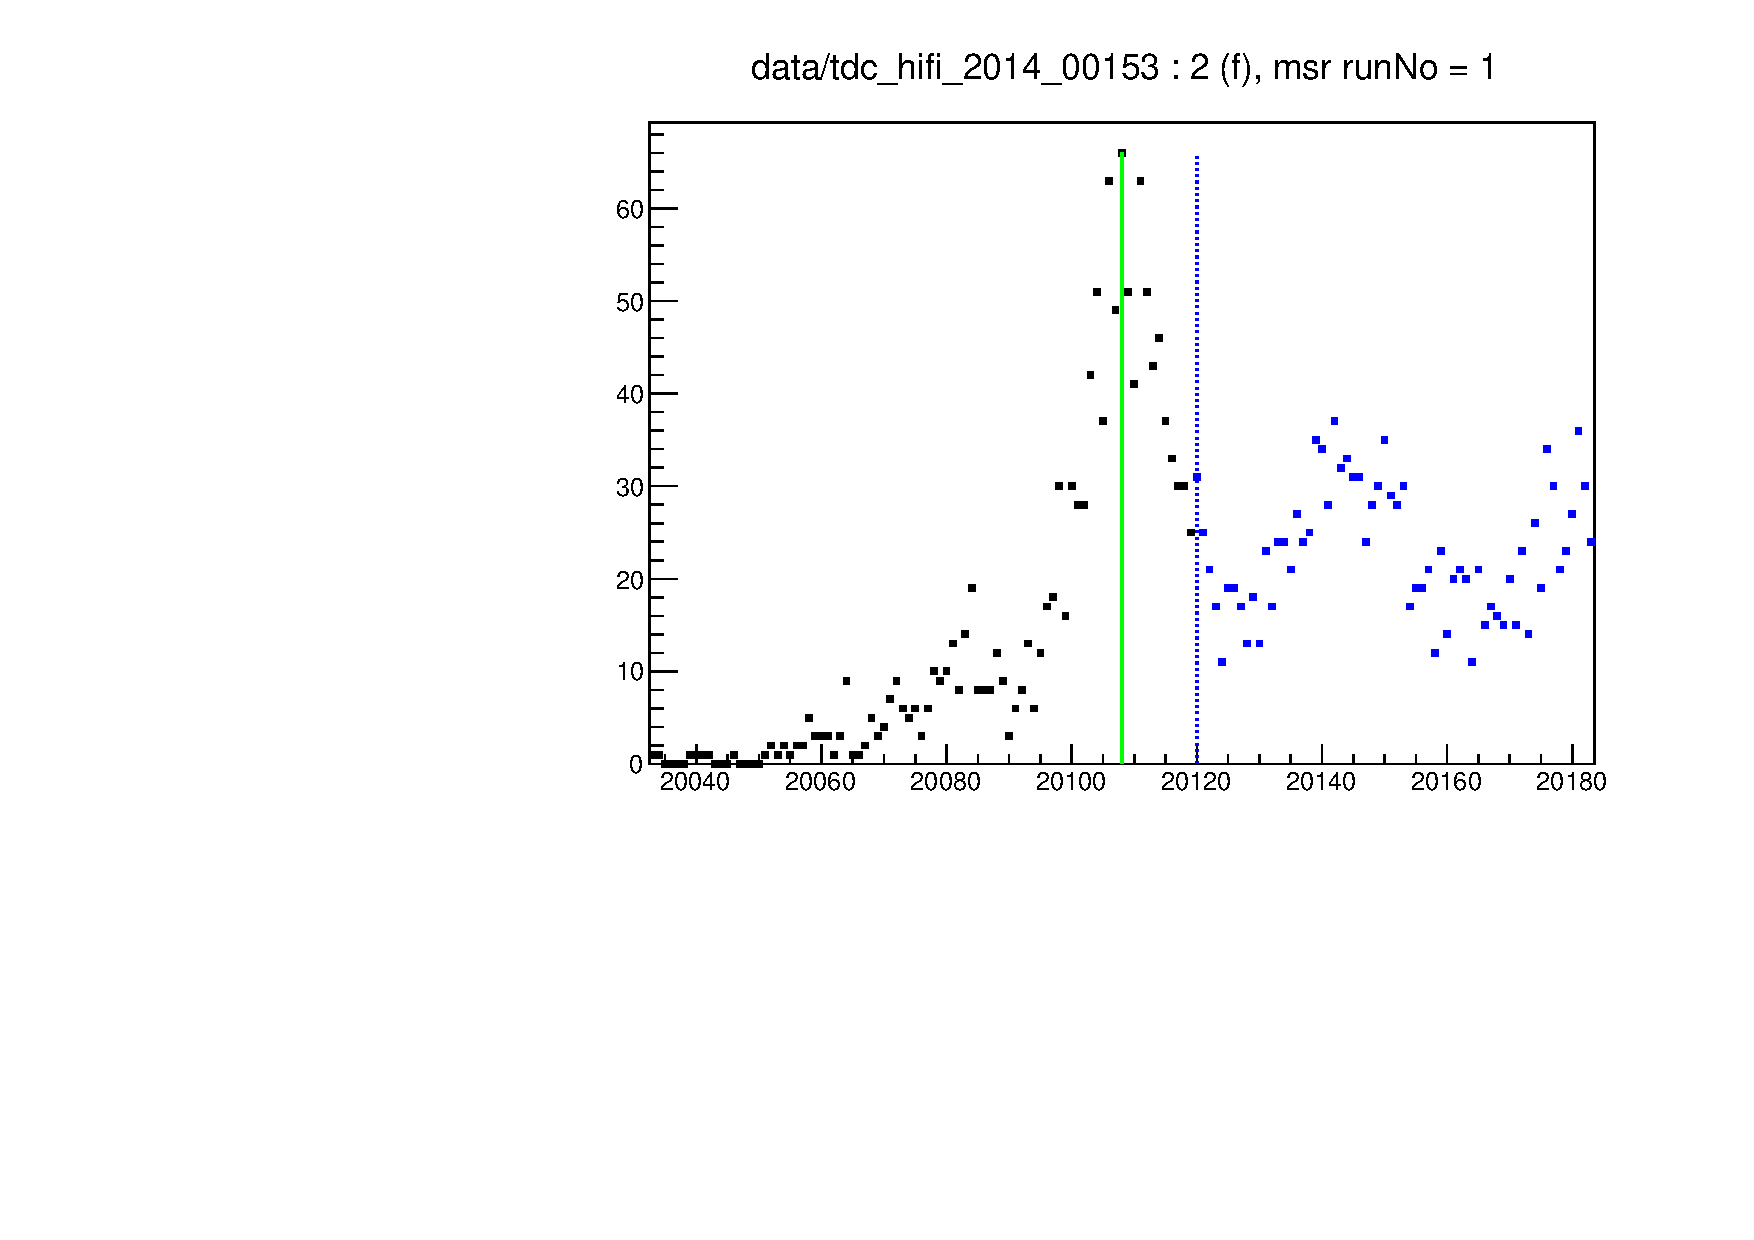
\includegraphics[width=0.5\textwidth]{HAL-9500-t0.pdf}
 \caption{The $t_0$ region of a typical HAL-9500 spectrum. The broad black hump with the green line, is the ``prompt'' peak.
          It is \emph{not} straight forward how to define $t_0$.}\label{fig:hal-9500-t0}
\end{figure}


\section{Discussion}

Both RRF transformation sketched above have weak points which makes it hard to estimate systematic errors. Both methods will fail at too
low fields of $\lesssim 1$T. The only and single purpose of the RRF transformation is slughish computer power! We developed GPU based fitting
which overcomes \emph{all} this uncontrolled weaknesses and henceforth RRF could be omitted altogether. I still added it for the time being,
since strong GPU/CPU hardware is still a bit costly and therefore not affordable to everyone.

In order to give a feeling about what might go ``wrong'' with the RRF, I was running a couple of test cases. The chosen asymmetry is

\begin{equation}\label{eq:asymmetry-simulation}
 A^{(j)}(t) =  A_0^{(j)} \sum_{k=1}^3 f_k \exp\left[-0.5\cdot (\sigma_k t)^2 \right] \cos(\gamma_\mu B_k t + \phi^{(j)}),
\end{equation}

\noindent with values found in Tab.\ref{tab:asymmetry-parameters}. For the simulation 4 positron detector signals were generated with 
$A_0^{(j)} = \left\{ 0.2554, 0.2574, 0.2576, 0.2566 \right\}$. The further ingredients were: $N_0^{(j)} = \left\{ 27.0, 25.3, 25.6, 26.9 \right\}$,
$N_{\rm bkg}^{(j)} = \left\{ 0.055, 0.060, 0.069, 0.064 \right\}$, and $ \phi^{(j)} = \left\{ 5.0, 95.0, 185.0, 275.0 \right\}$.

\begin{table}[h]
 \centering
 \begin{tabular}{c|c|c|c}
   $k$ & $f_k$ & $\sigma_k$ & $B_k$ \\ 
       &       & ($1/\mu$s) & (T)   \\ \hline\hline
    1  & 0.5   & 7          & $1$ or $9$ \\
    2  & 0.2   & 0.75       & $1.02$ or $9.02$ \\
    3  & 0.3   & 0.25       & $1.06$ or $9.06$
 \end{tabular}
 \caption{Parameters used in Eq.(\ref{eq:asymmetry-simulation}).}\label{tab:asymmetry-parameters}
\end{table}
 
\begin{figure}[h]
 \centering
 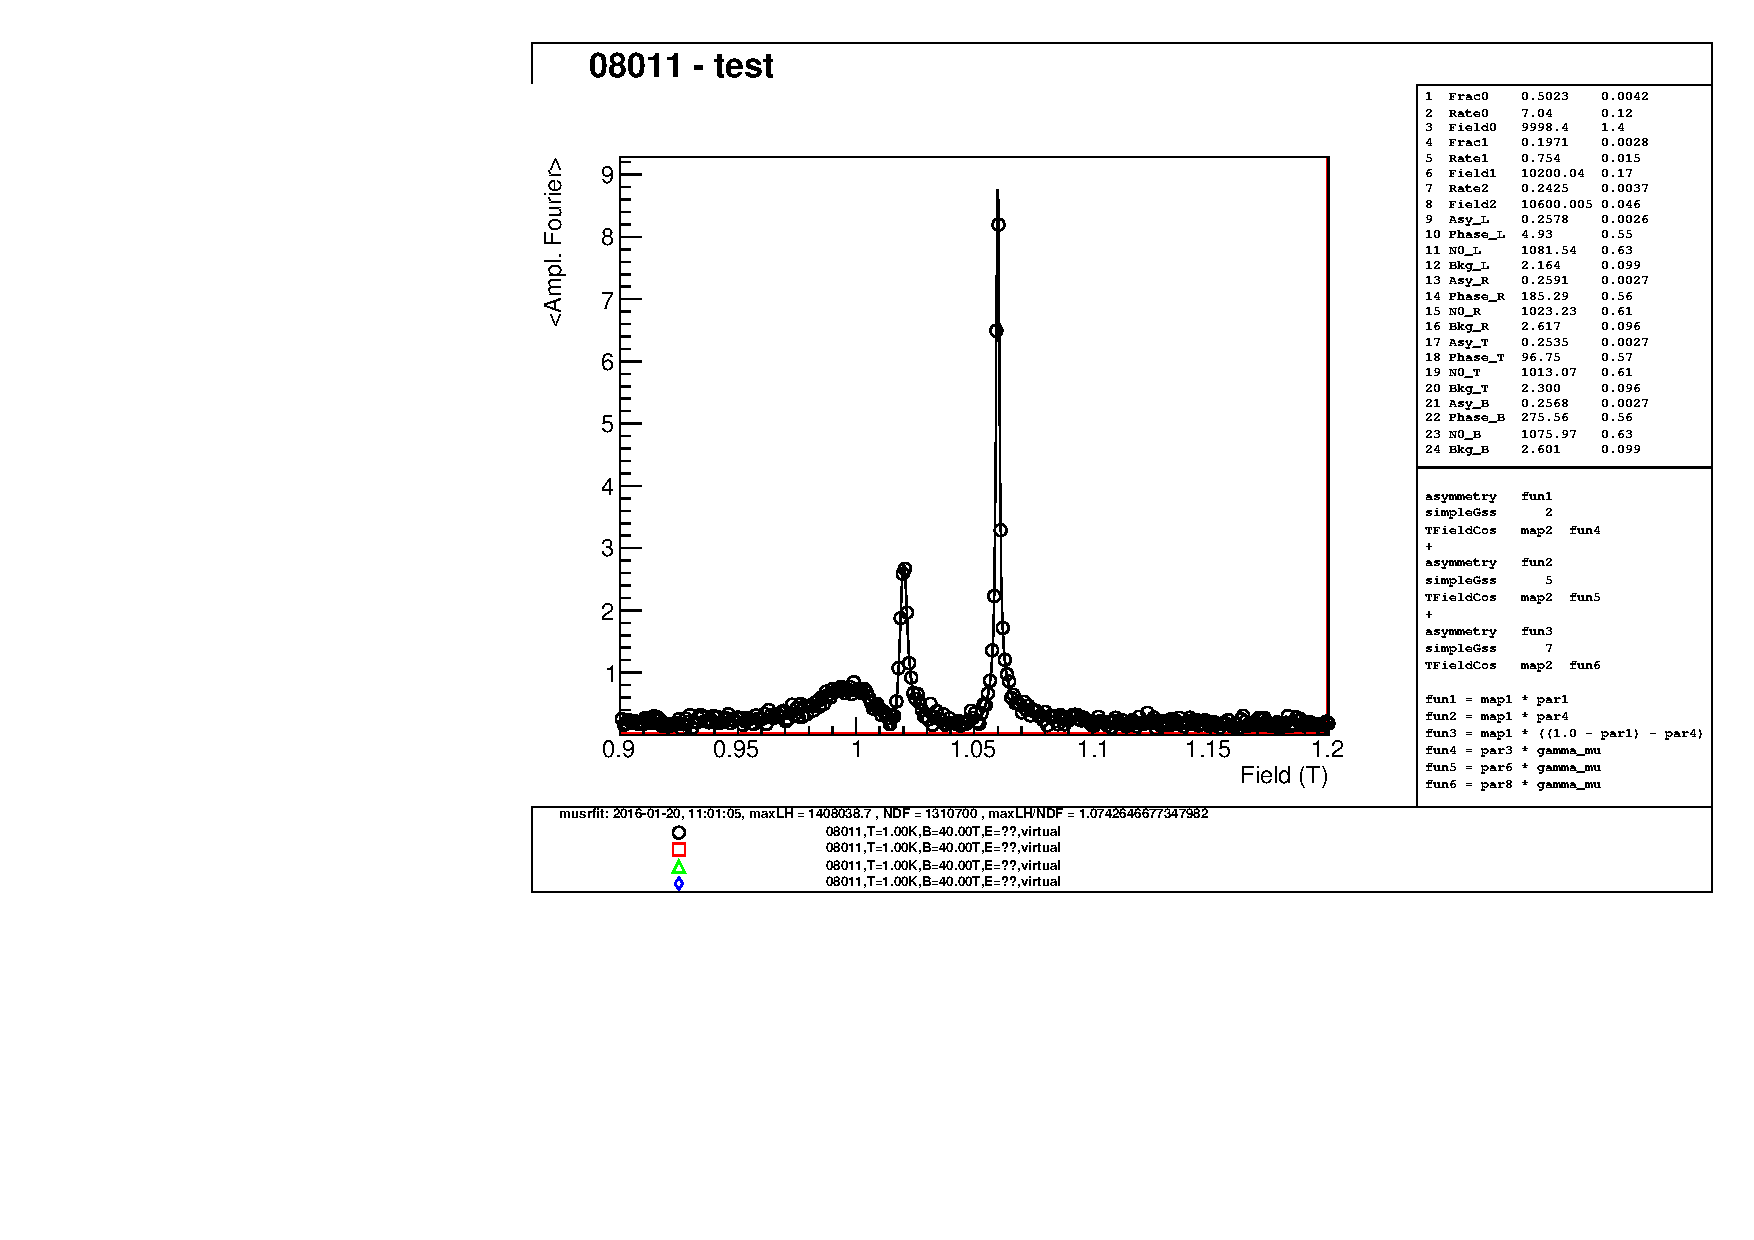
\includegraphics[width=0.45\textwidth]{08011-Fourier-Averaged.pdf} \quad
 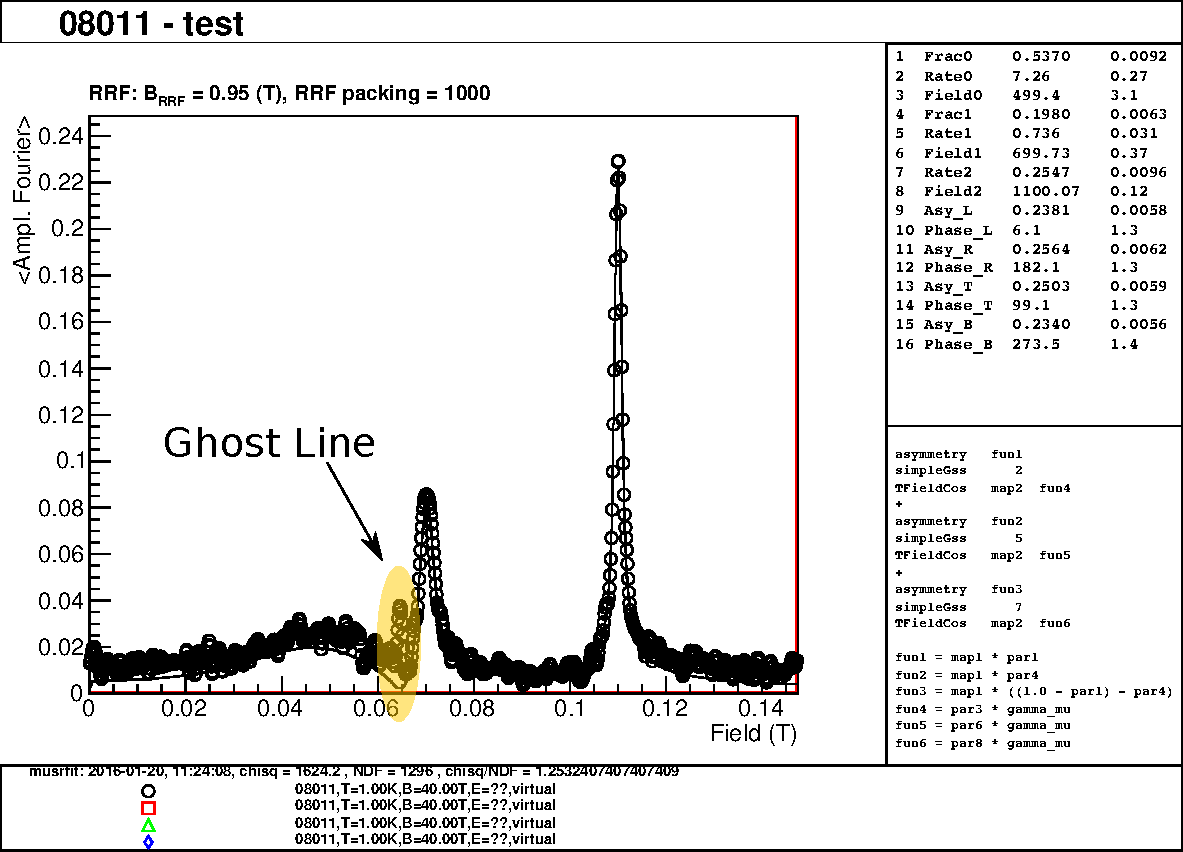
\includegraphics[width=0.45\textwidth]{08011-RRF-Histo-Fourier-Averaged-Ghost.pdf} \\
 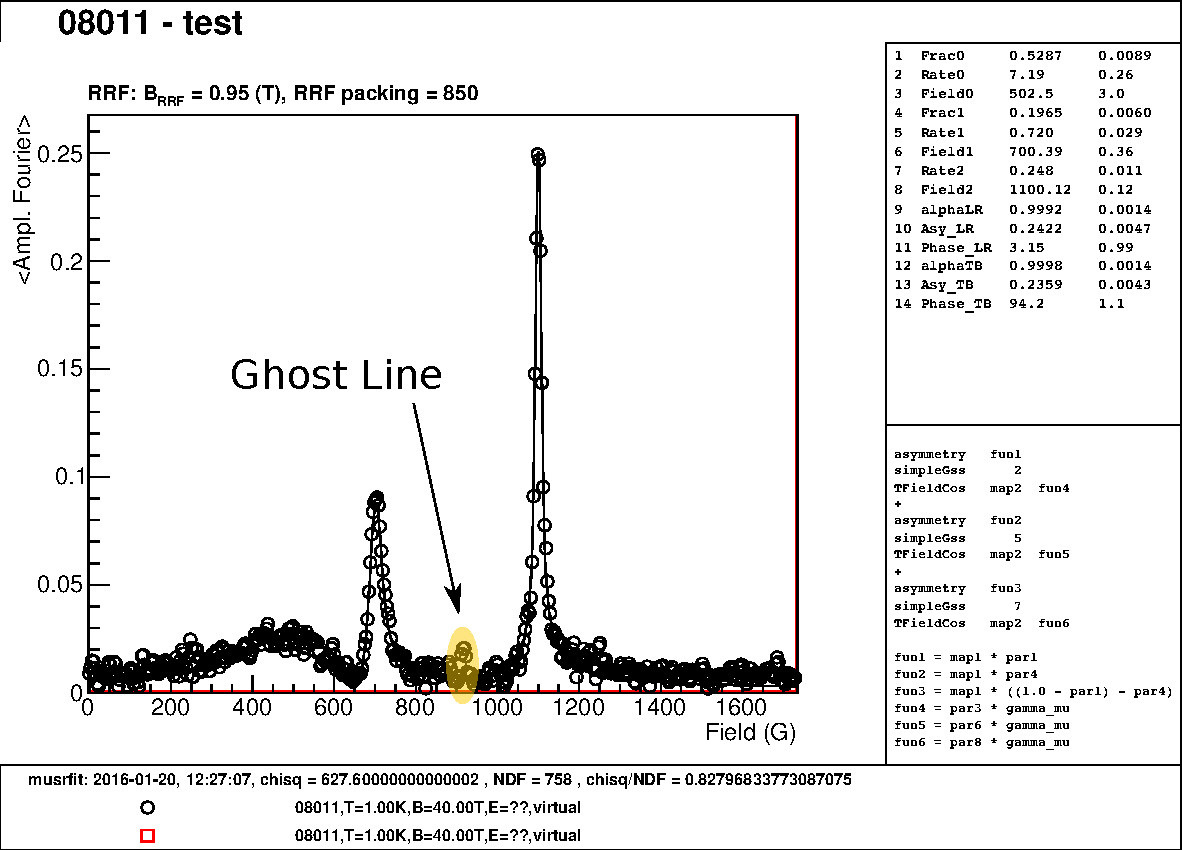
\includegraphics[width=0.45\textwidth]{08011-RRF-Asym-Fourier-Averaged-Ghost.pdf}
 \caption{Averaged Fourier power spectra. Top left: from single histogram fit for the 1T data set. 
          Top right: from single histogram RRF fit. Bottom: from asymmetry RRF fit. Both RRF
          sets show ghost lines.}\label{fig:08011-Fourier}
\end{figure}

Figure.\ref{fig:08011-Fourier} shows the averaged Fourier power spectra for the simulated data sets at 1T. Both RRF transformation are
showing ghost lines, even for optimally chosen RRF rebinning. At higher fields this is less pronounced. The ghost lines have various origins 
such as aliasing effects due to the RRF packing not prefectly suppressing the high frequency part of $A_{\rm rrf}(t)$, leakage of the RRF frequency 
for not sufficently precise known $N_0$ (see Eq.(\ref{eq:N0-rrf})) for single histogram RRF fits, etc.

Fits of simulated data as described above (see Eq.(\ref{eq:asymmetry-simulation}), with fields 0.5, 1.0, 3.0, 5.0, 7.0, and 9.0T) show that above 
about 1T the model parameters of the RRF fits are acceptable, but the error bars are typically about a factor 3 larger compared to single histogram
fits. The asymmetries of the RRF fits are ``substantially'' too small. The $\chi^2$ values are close to meaningless for the RRF fits, since they
are strongly depending on the RRF packing, time interval chosen, etc. 

To summaries: RRF fits can be used for online analysis if no GPU accelerator is available, but \emph{must not} be used for any final analysis!

\bibliographystyle{amsplain}
\bibliography{rrf}

\end{document}